\section{Базовые морфологические операции}
\subsection{Исходное изображение}

Для первого задания выберем фотографию Яна Берри, сделанную в разгар событий Пражской весны:
\begin{figure}[ht!]
    \centering
    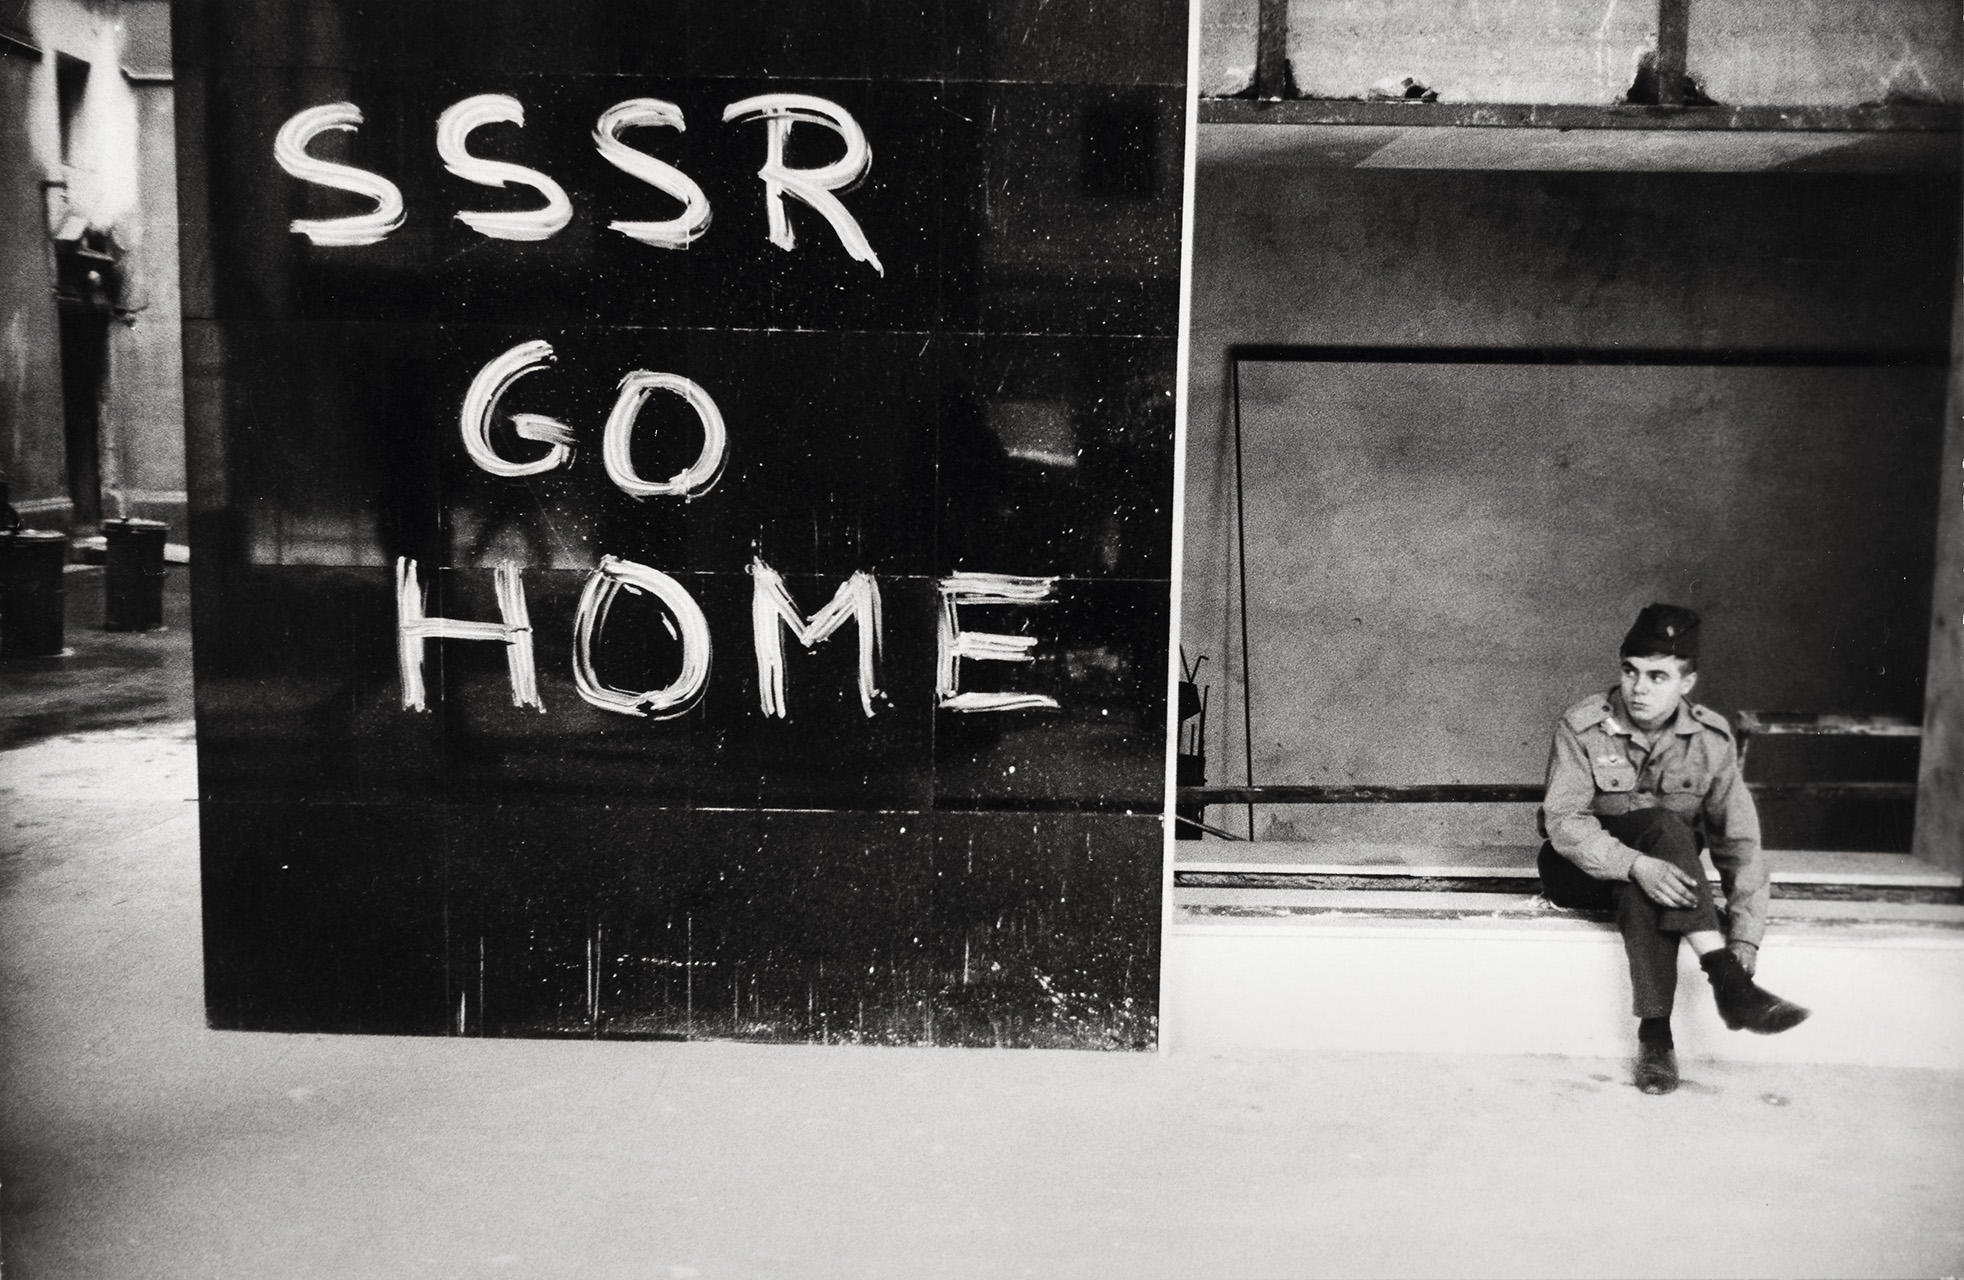
\includegraphics[width=\textwidth]{images/source_images/Ian_Berry_A young_Russian soldier.jpg}
    \caption{Ян Берри. Молодой советский солдат отдыхает рядом с плакатом <<СССР, возвращайся домой>> на Вацлавской площади. Прага, Чехословакия. 1968}
    \label{img:Soldier_orig}
\end{figure} 

Нашей задачей будет минимизация дефектов формы на надписи \textit{SSSR GO HOME}. В этом нам поможет \textit{Python}. Для начала загрузим изображение и выберем область изображения с надписью для выполения преобразований.

\begin{lstlisting}[caption={Исходный код для считывания изображения}, label={lst:img_reading}]
    # loading grayscale image
    src_img = cv.imread('source_images/Ian_Berry_A young_Russian soldier.Jpeg', 0)
    assert src_img is not None, "File could not be read"
    result = np.copy(src_img)
    # selecting specific area
    spec_area = src_img[0:735, 200:1080]
\end{lstlisting}

\begin{figure}[ht!]
    \centering
    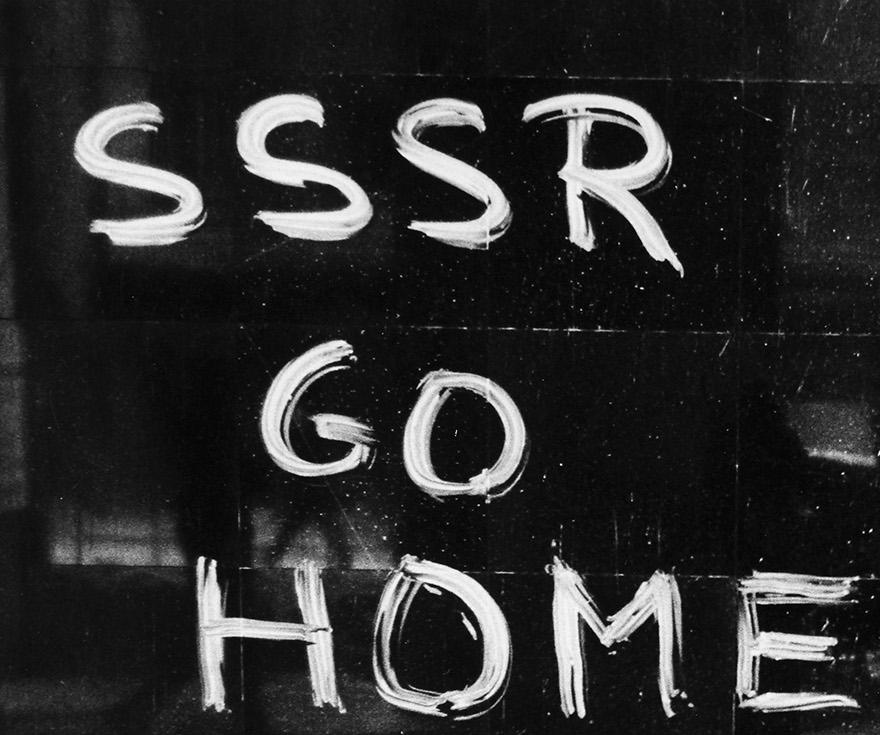
\includegraphics[width=0.7\textwidth]{images/transformed_images/1/Caption.jpg}
    \caption{Надпись, которая подвергнется преобразованиям}
    \label{img:Caption_orig}
\end{figure} 

С помощью эрозии избавимся от лишних точек на стене и выступов на буквах. Далее применим дилатацию от избавления от <<внутренних дырок>> и затем эрозию для избавления от частиц, появившихся в результате дилатации, и возвращения буквам их исходной толщины.

\begin{lstlisting}[caption={Исходный код для преобразования надписи}, label={lst:morphological}]
    # morphological operations
    disk = cv.getStructuringElement(cv.MORPH_ELLIPSE, (3, 3))
    erosion = cv.erode(spec_area, disk, iterations=1)
    dilation = cv.dilate(erosion, disk, iterations=7)
    erosion2 = cv.erode(dilation, disk, iterations=5)
\end{lstlisting}
\begin{figure}
    \centering
    \begin{subfigure}[b]{0.3\textwidth}
        \centering
        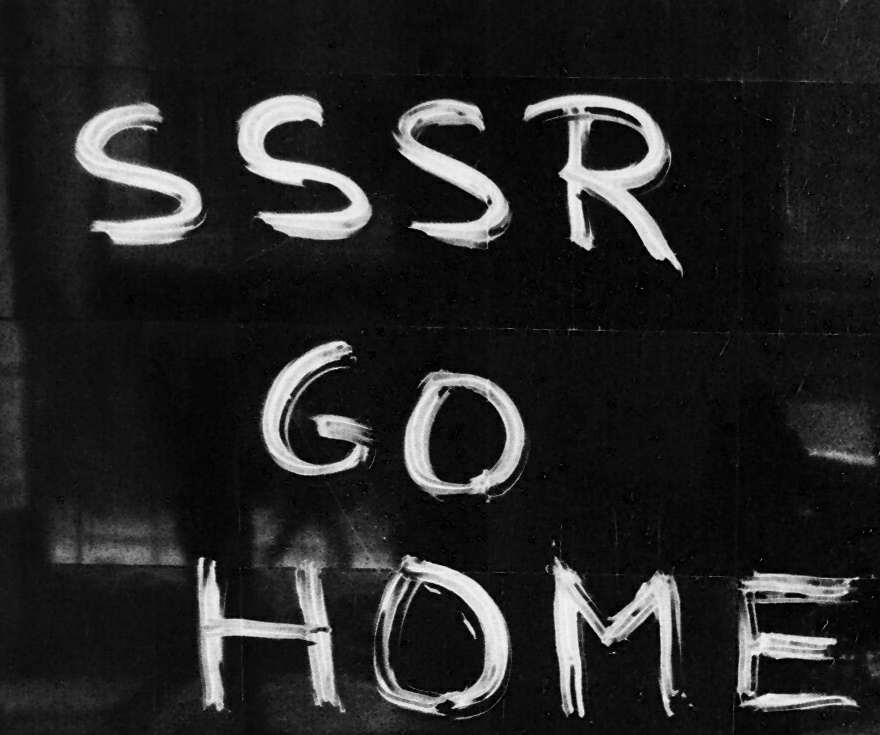
\includegraphics[width=\textwidth]{images/transformed_images/1/4 try/Erosed_1.jpg}
        \caption{}
        \label{img:Caption_erosed_1}
    \end{subfigure}
    \begin{subfigure}[b]{0.3\textwidth}
        \centering
        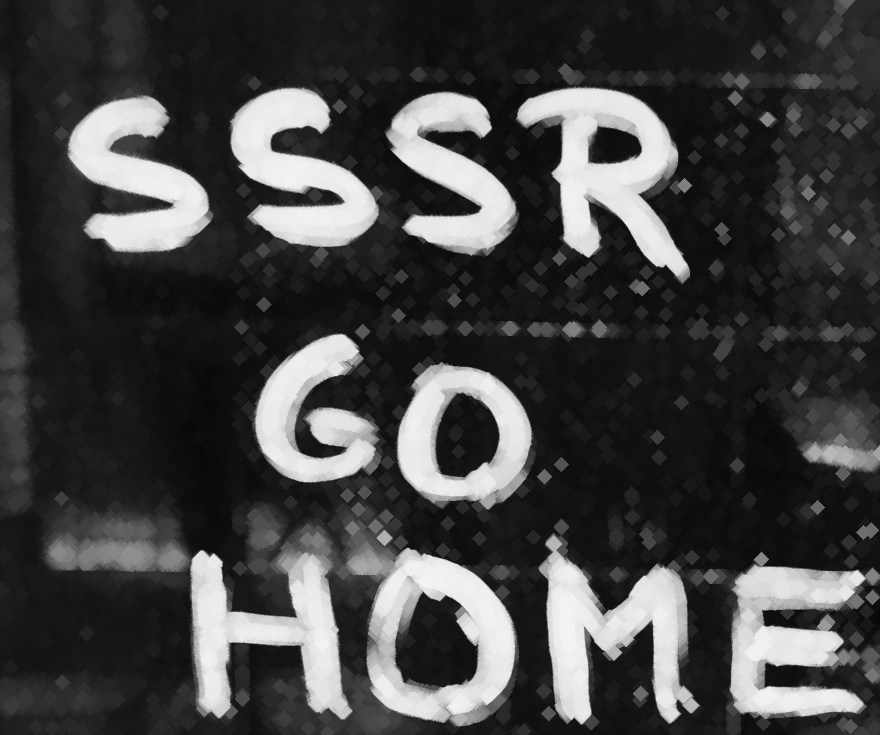
\includegraphics[width=\textwidth]{images/transformed_images/1/4 try/Dilation_7.jpg}
        \caption{}
        \label{img:Caption_dilation}
    \end{subfigure}
    \begin{subfigure}[b]{0.3\textwidth}
        \centering
        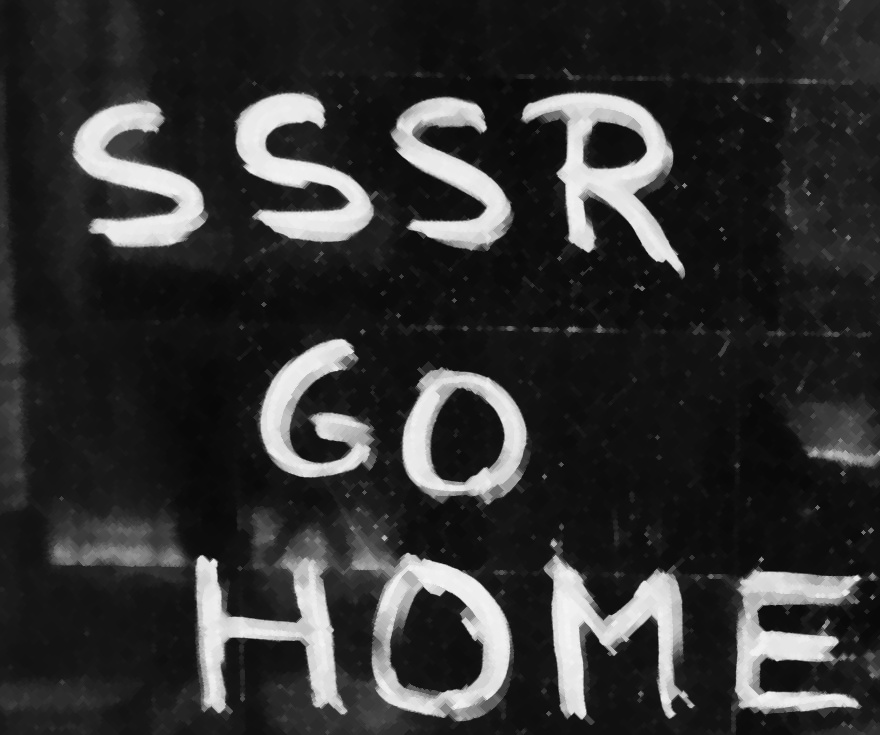
\includegraphics[width=\textwidth]{images/transformed_images/1/4 try/Erosed_2_5.jpg}
        \caption{}
        \label{img:Caption_erosed_2}
    \end{subfigure}
    \caption{Избавление от дефектов: (а) результат применения эрозии, (b)  результат применения дилатации 7 раз, (c)  результат применения эрозии 5 раз}
    \label{img:Transforms}
\end{figure}
\clearpage

\subsection{Результаты}

После преобразований необходимо вернуть <<новую>> надпись в исходное изображение.

\begin{lstlisting}[caption={Исходный код для получения итогового изображения}, label={lst:result}]
    # displaying transformed image
    result[0:735, 200:1080] = erosion2
    display_image('Result', result, 1)
\end{lstlisting}

\begin{figure}[ht!]
    \centering
    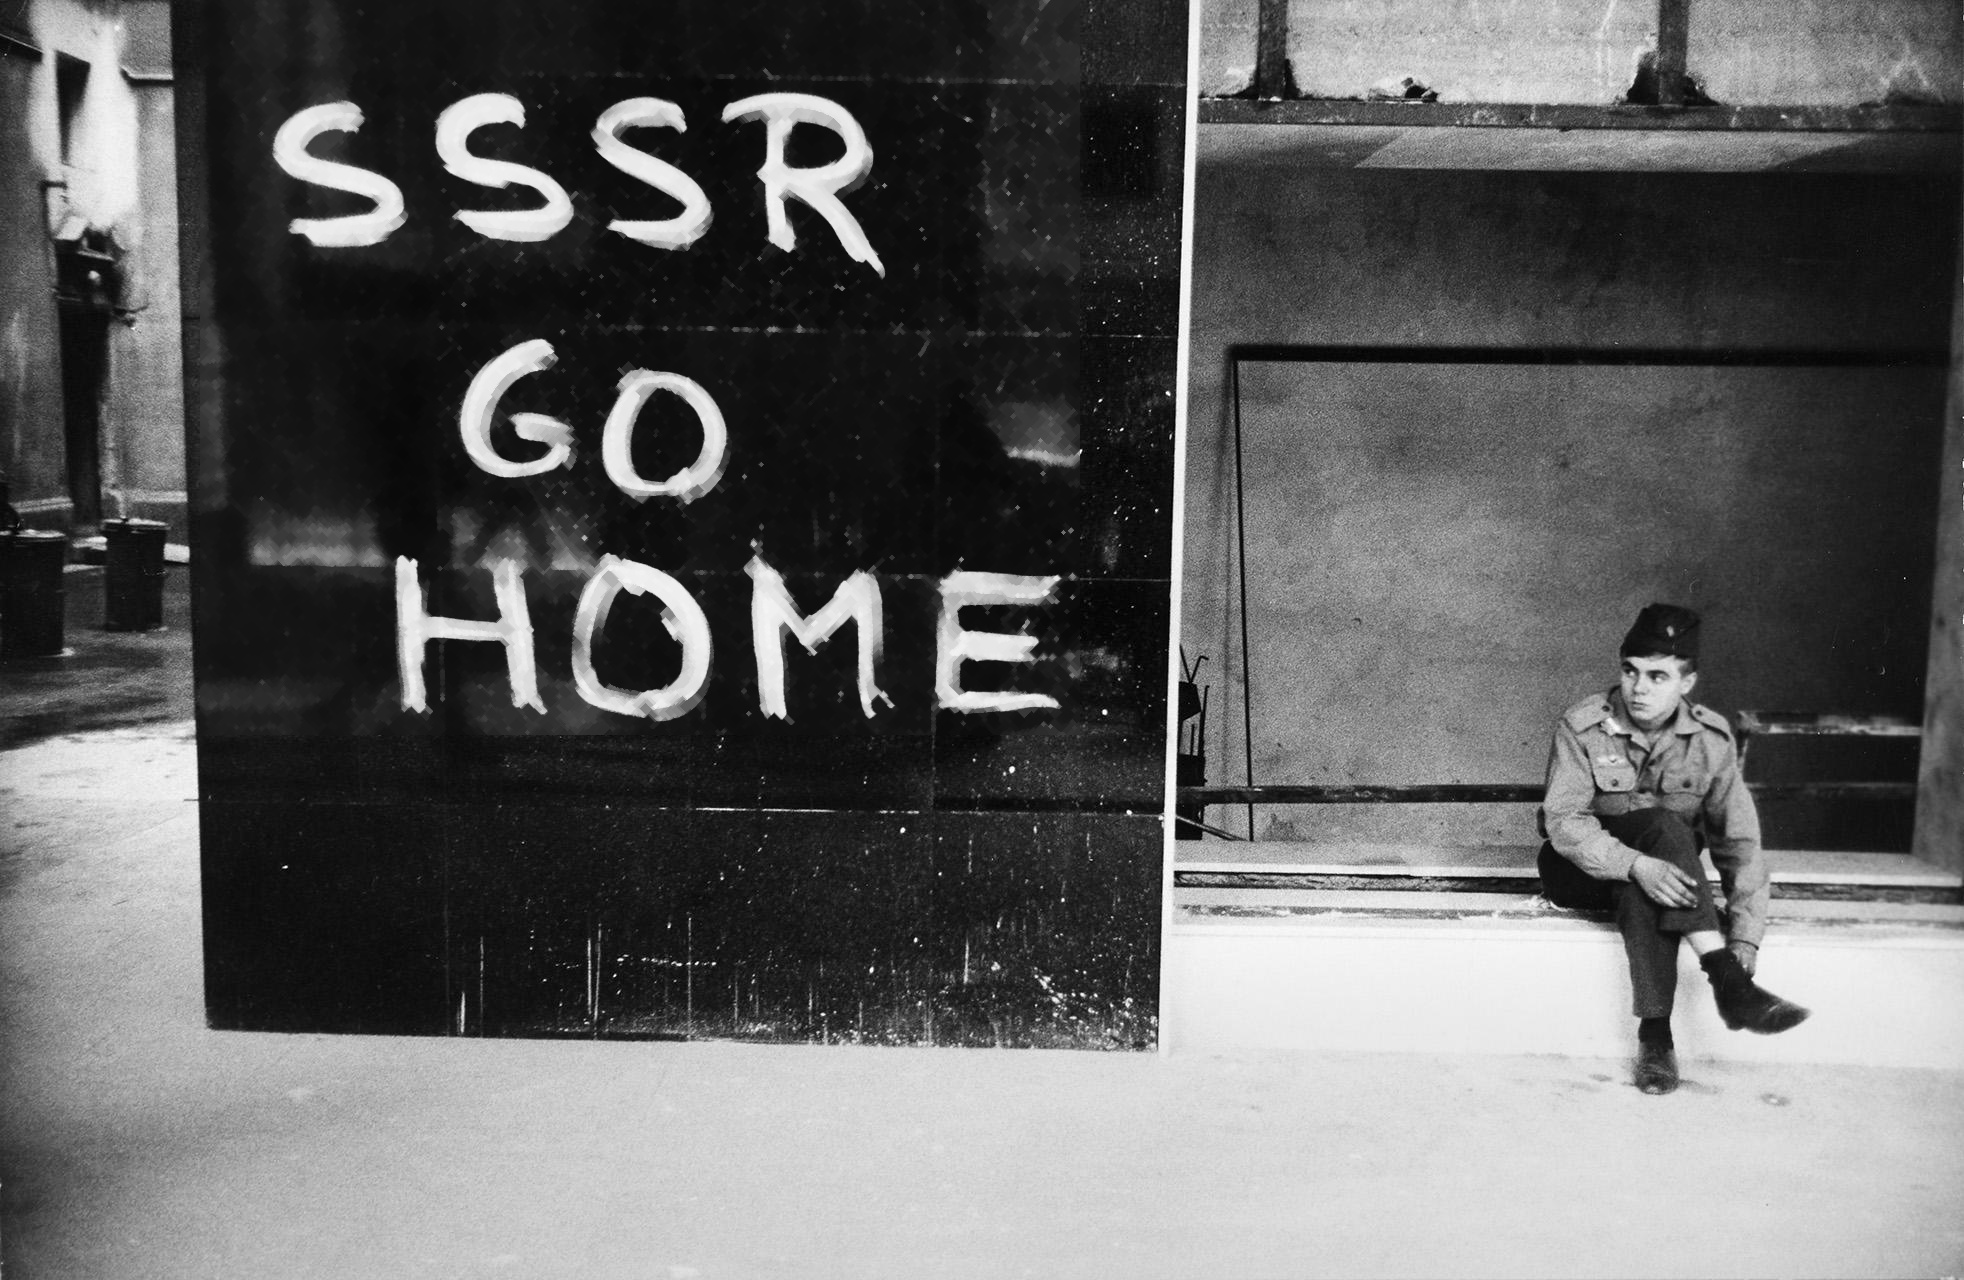
\includegraphics[width=\textwidth]{images/transformed_images/1/4 try/Result.jpg}
    \caption{Результат применения базовых морфологических операций}
    \label{img:Soldier_result}
\end{figure} 



\newpage
\section{Разделение объектов}
\subsection{Исходное изображение}

Обратимся к кругам и их производным. Исходное изображение:

\begin{figure}[ht!]
    \centering
    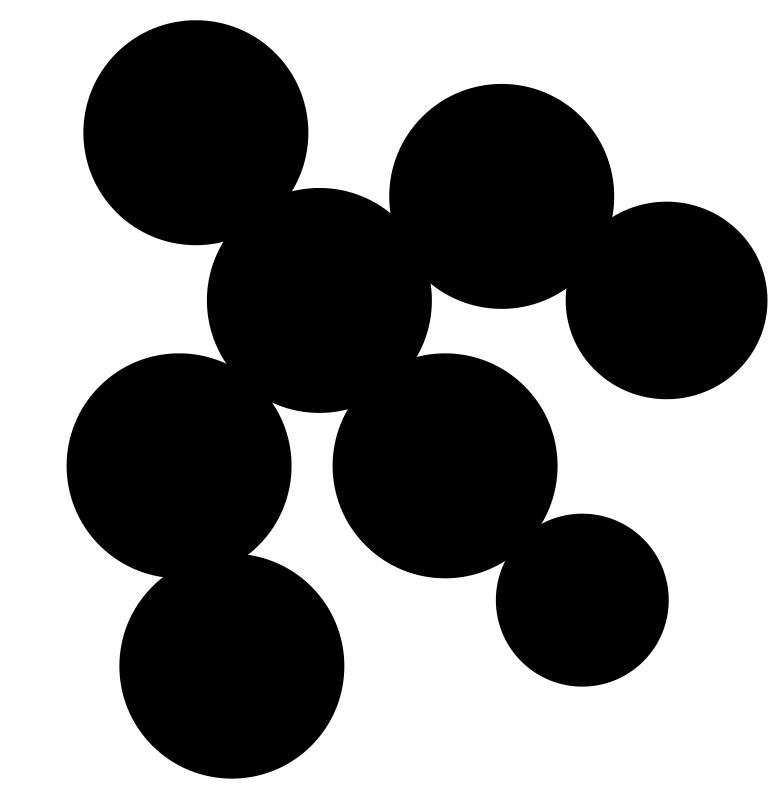
\includegraphics[width=0.5\textwidth]{images/source_images/circles.jpg}
    \caption{Круги}
    \label{img:circles_orig}
\end{figure} 

Для выполнения этого задания воспользуемся \textit{MATLAB}.

\subsection{Программа на языке MATLAB}

\begin{lstlisting}[caption={Исходный код программы для разделения объектов}, label={lst:separation}]
    src_img = imread("circles.jpg");
    gray_img = im2gray(src_img);
    BW = imbinarize(gray_img);
    BW = ~BW;
    imwrite(BW,"binary_inv.jpg");
    BW2 = bwmorph(BW,'erode',45);
    imwrite(BW,"erosed.jpg");
    BW2 = bwmorph(BW2,'thicken',Inf);
    imwrite(BW,"boundaries.jpg");
    BW = ~(BW & BW2);
    imwrite(BW,"result.jpg");
\end{lstlisting}

\subsection{Результаты}

\newpage
\section{Сегментация}
\subsection{Исходное изображение}

Для последнего задания выберем следующее изображение:

\begin{figure}[ht!]
    \centering
    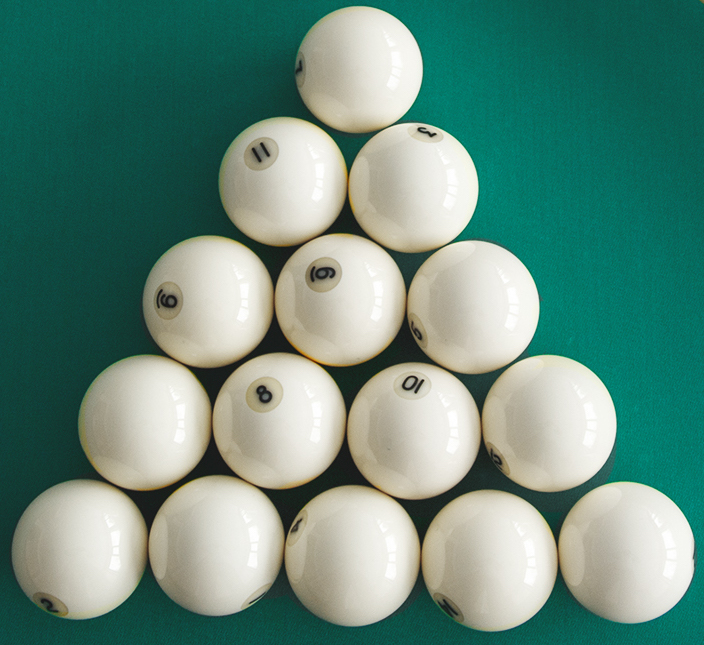
\includegraphics[width=0.8\textwidth]{images/source_images/snooker.jpg}
    \caption{Шары для игры в бильярд}
    \label{img:billiard_balls}
\end{figure} 

\subsection{Программа на языке Python}
\begin{lstlisting}[caption={Исходный код программы для сегментации изображения}, label={lst:separation}]
    def bwareaopen(image, dim, conn=8):
        assert image.ndim == 2, None
        # Find all connected components
        num, labels, stats, centers = cv.connectedComponentsWithStats(image, connectivity=conn)
        # Check size of all connected components
        for i in range(num):
            if stats[i, cv.CC_STAT_AREA] < dim:
                image[labels == i] = 0
        return image


    # loading an image
    src_img = cv.imread('source_images/snooker.jpg')
    # converting it to binary
    gray_img = cv.cvtColor(src_img, cv.COLOR_BGR2GRAY)
    ret, i_bw = cv.threshold(gray_img, 0, 255, cv.THRESH_BINARY + cv.THRESH_OTSU)
    # deleting tiny connected components
    i_bw = bwareaopen(i_bw, 20, 8)
    disk = cv.getStructuringElement(cv.MORPH_ELLIPSE, (5, 5))
    i_bw = cv.morphologyEx(i_bw, cv.MORPH_CLOSE, disk)
    # display_image('Binary_closed', i_bw, 1)

    # finding foreground
    i_fg = cv.distanceTransform(i_bw, cv.DIST_L2, 5)
    ret1, i_fg = cv.threshold(i_fg, 0.6 * i_fg.max(), 255, 0)
    i_fg = i_fg.astype(np.uint8)
    ret2, markers = cv.connectedComponents(i_fg)
    # display_image('Fg', i_fg, 1)


    # Find background location
    i_bg = np.zeros_like(i_bw)
    markers_bg = markers.copy()
    markers_bg = cv.watershed(src_img, markers_bg)
    i_bg[markers_bg == -1] = 255
    # display_image('Bg', i_bg, 1)

    # Define undefined area
    i_unk = cv.subtract(i_bg, i_fg)
    # Define all markers
    markers = markers + 1
    markers[i_unk == 255] = 0
    # Do watershed
    # Prepare for visualization
    markers = cv.watershed(src_img, markers)
    # display_image('UND', i_unk, 1)
    markers_jet = cv.applyColorMap((markers.astype(np.float32)*255/(ret2 + 1)).astype(np.uint8), cv.COLORMAP_JET)
    display_image('Jet_fg_markers', markers_jet, 1)
    src_img[markers == -1] = (0, 0, 255)
    # display_image('result', src_img, 1)
\end{lstlisting}

\subsection{Результат}

Для начала необходимо получить бинарное изображение, предварительно удалив лишние детали.

\begin{figure}[ht!]
    \centering
    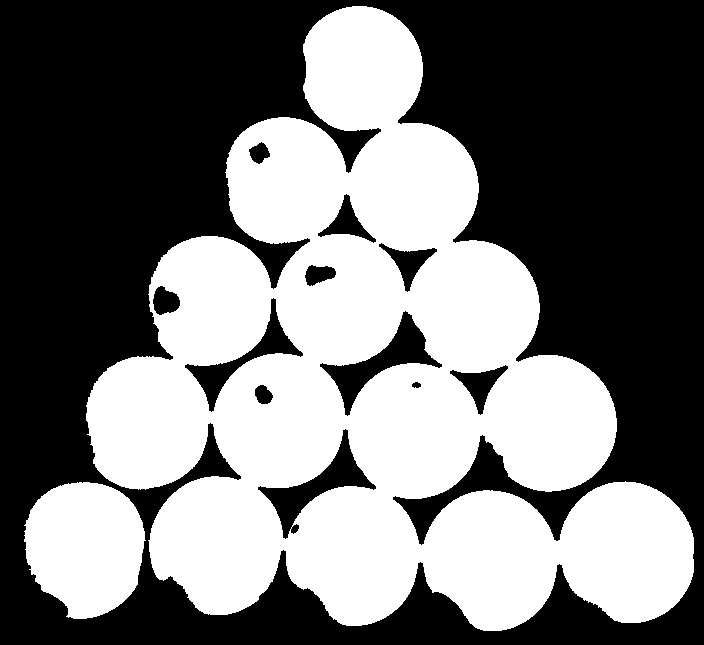
\includegraphics[width=0.7\textwidth]{images/transformed_images/3/Binary_closed.jpg}
    \caption{Бинарное изображение}
    \label{img:bin_balls}
\end{figure} 

Далее воспользуемся преобразованием евклидова расстояния и после дополнительной фильтрации получим маркеры переднего плана:

\begin{figure}[ht!]
    \centering
    \begin{subfigure}{0.4\textwidth}
        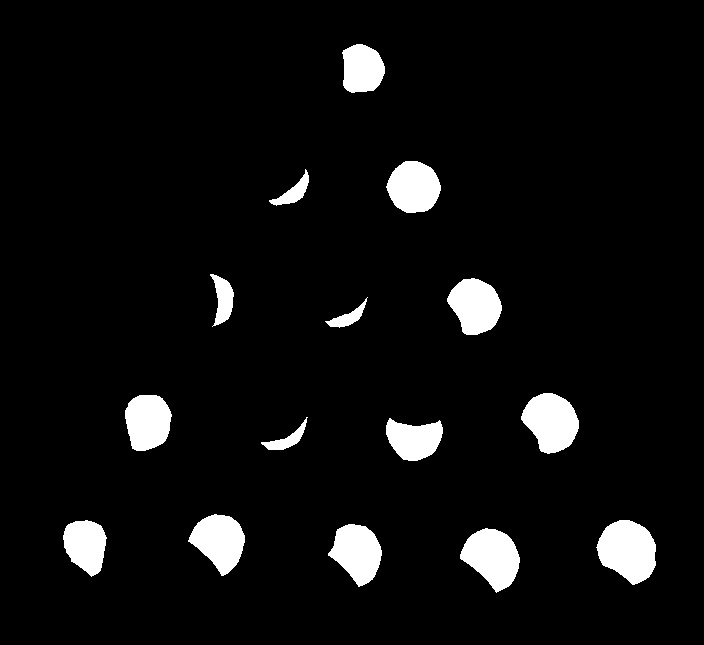
\includegraphics[width=\textwidth]{images/transformed_images/3/Fg.jpg}
        \caption{}
        \label{img:bin_fg}
    \end{subfigure}
    \begin{subfigure}{0.4\textwidth}
        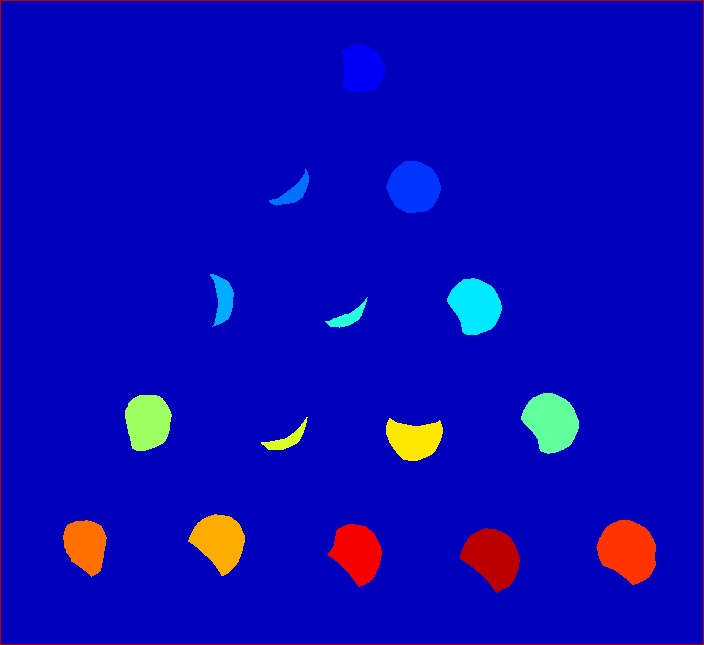
\includegraphics[width=\textwidth]{images/transformed_images/3/Jet_fg_markers.jpg}
        \caption{}
        \label{img:jet_fg}
    \end{subfigure}
    \caption{Определение маркеров переднего плана: (a) область маркеров переднего плана, (b) маркеры переднего плана}
    \label{img:FG}
\end{figure} 

Далее получим маркеры фона и неопределенной области:

\begin{figure}[ht!]
    \centering
    \begin{subfigure}{0.4\textwidth}
        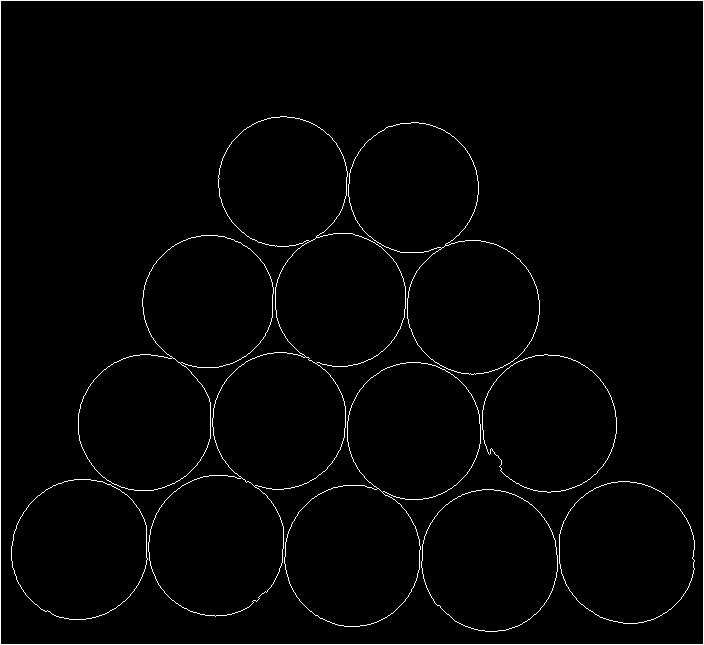
\includegraphics[width=\textwidth]{images/transformed_images/3/Bg.jpg}
        \caption{}
        \label{img:bin_bg}
    \end{subfigure}
    \begin{subfigure}{0.4\textwidth}
        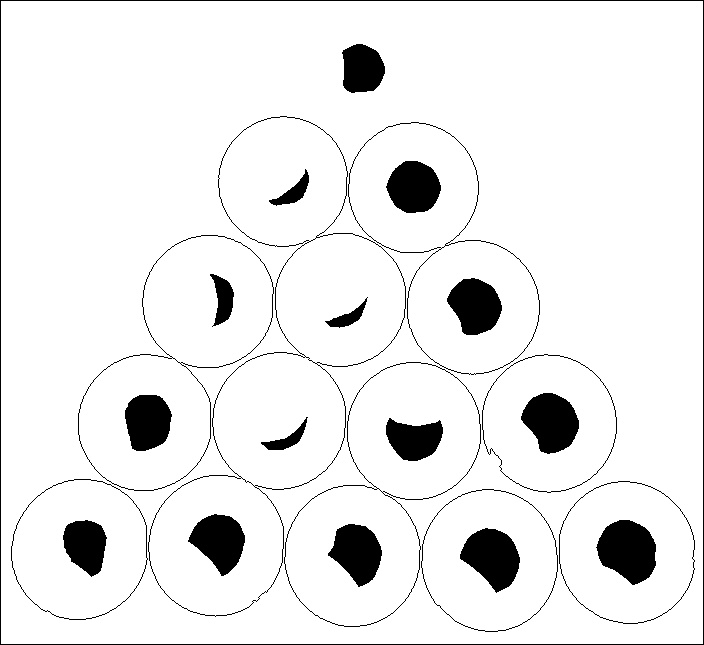
\includegraphics[width=\textwidth]{images/transformed_images/3/UND.jpg}
        \caption{}
        \label{img:bin_und}
    \end{subfigure}
    \caption{Определение маркеров: (a) фона, (b) неопределенной области}
    \label{img:BG}
\end{figure} 

Наконец, получим результаты сегментации:

\begin{figure}[ht!]
    \centering
    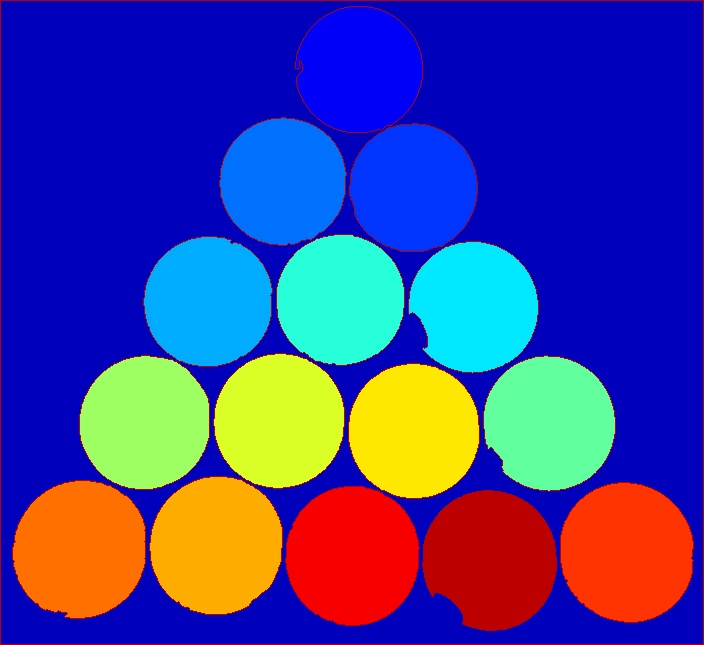
\includegraphics[width=0.7\textwidth]{images/transformed_images/3/Jet.jpg}
    \caption{Результат сегментации}
    \label{img:seg}
\end{figure} 
\clearpage
\begin{figure}[ht!]
    \centering
    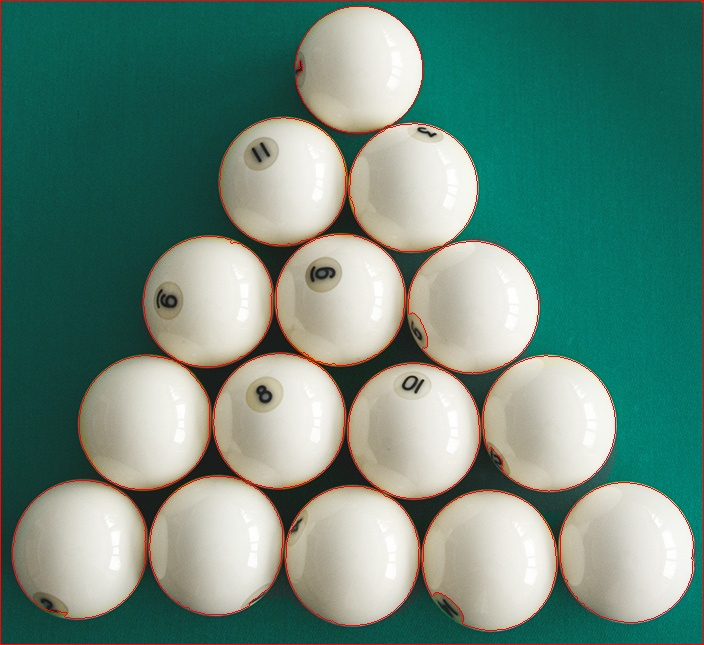
\includegraphics[width=0.7\textwidth]{images/transformed_images/3/result.jpg}
    \caption{Результат сегментации, наложенный на исходное изображение}
    \label{img:seg_orig}
\end{figure} 

\newpage
\section{Выводы}

В результате выполнения работы мы познакомились с морфологическими операциями, а также рассмотрели задачи, для решения которых они применяются. С помощью Морфологических операций нам удалось минимизировать дефекты формы (рис. \ref{img:Soldier_result}), разделить <<склееные>> объекты (рис. \ref{img:result_circles}) и сегментировать изображение (рис. \ref{img:seg_orig}).

Полный код программы и изображения можно найти на \href{https://github.com/NikBrat/ComputerVision_Lab6}{GitHub}.

\section{Ответы на вопросы}

\newcounter{question}
\setcounter{question}{0}

\newcommand{\question}[1]{\item[Q\refstepcounter{question}\thequestion.] #1}
\newcommand{\answer}[1]{\item[A\thequestion.] #1}


\begin{itemize}

    \question{Включает ли результат открытия в себя результат закрытия?}
   
    \answer{Нет. Правильнее будет сказать, что результат \textbf{закрытия} включает в себя результат \textbf{открытия}}
    
    \question{Какой морфологический фильтр необходимо применить, чтобы убрать у объекта выступы?}
    \answer{Для того, чтобы убрать лишние выступы, можно использовать \textbf{эрозию}, однако это приведет к уменьшению размера объекта. Поэтому можно также воспользоваться операцией \textbf{открытия}, благодаря которой мы сможем избавиться от выступов и сохранить размеры объекта. Единственный недостаток этого подхода -- острые углы будут становится более округлыми.} 

    \question{Каким образом с помощью морфологических операций можно найти контур объекта?}
    \answer{ Для нахождения контура объекта нам необходимо, в превую очередь, получить бинарное изображение этого объекта. Далее мы должны вычесть (по правилам теории множеств) из результата \textbf{дилатации} исходное изображение, получив при этом внешний контур объекта. Для получения внутреннего контура необходимо из исходного изображения вычесть результат \textbf{эрозии}.}

    \question{Что такое морфология?}
    \answer{Дословно слово \textit{морфология} переводится как наука о форме. Вообще говоря, морфология -- это теория анализа и обработки геометрических фигур, основанная на теории множеств и топологии.}
\end{itemize}

\section{P.S.}

Так это лабораторная знаменует собой окончание курса, то наша команда, в качестве благодарности, приготовила свои изображения:

\begin{figure}[ht!]
    \centering
    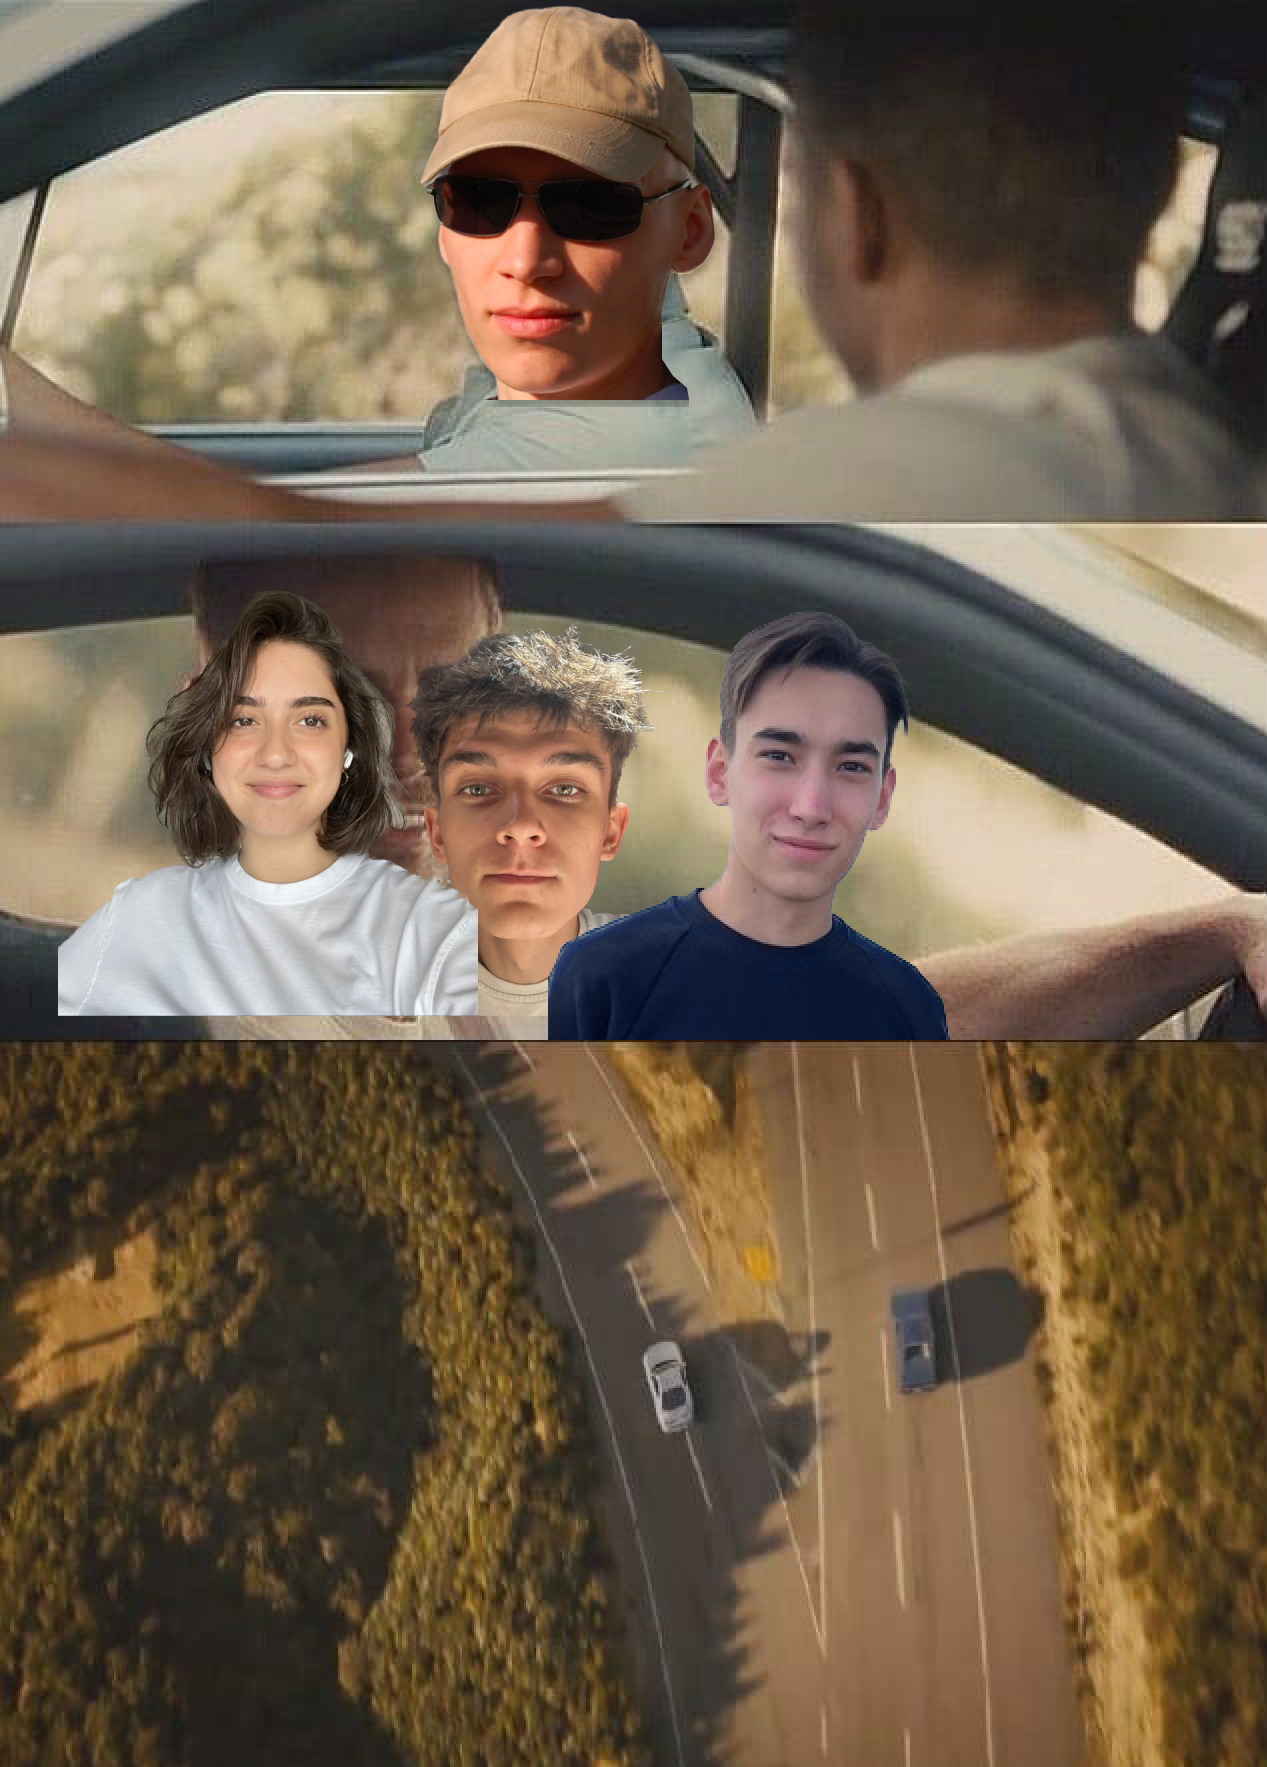
\includegraphics[width=0.8\textwidth]{images/image 1.png}
    \label{img:fast}
\end{figure} 

\begin{figure}[ht!]
    \centering
    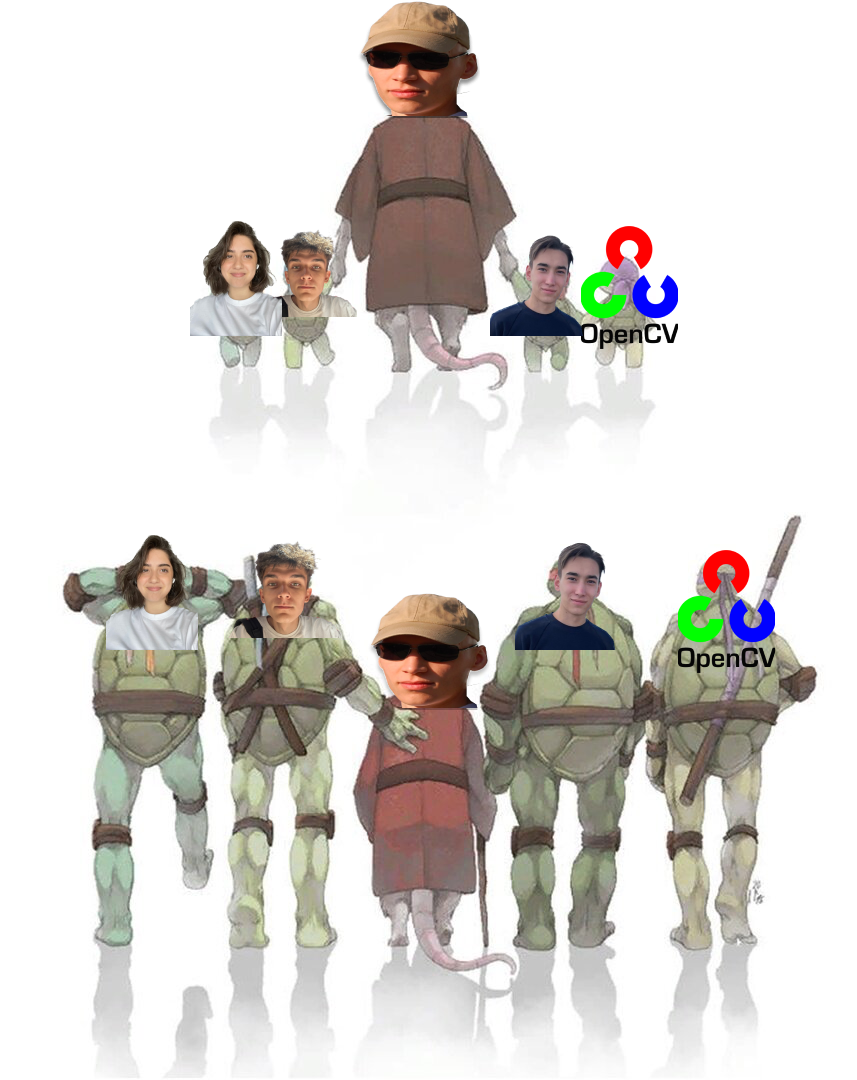
\includegraphics[width=0.8\textwidth]{images/Component 1.png}
    \label{img:turtles}
\end{figure} 